\section{引言}
\subsection{问题背景}

热风烘干通过外界对流换热提高药材温度，并通过表面传质持续移走水分。热量与水分在材料内部的传播速率不同，且物性会随温度和含水率变化；在长时间烘干中，材料收缩还会改变传递距离和面积体积比。因此，只给出平均温度或经验干燥曲线，难以回答“内部各处何时均达到安全含水率”这一问题。热质耦合、变物性与收缩几何均是干燥建模中的常见关键因素\cite{caccavale2016,rahman2007,aprajeeta2015}。

题目给出长度$25$ cm、初始半径$2$ cm的圆柱药材，初温为$28\ ^\circ\mathrm C$，初始干基含水率为$2.55\ \mathrm{kg/kg}$；附件给出烘房温度、环境水分量以及随时间变化的药材半径。本文的任务不是拟合一条总体曲线，而是求解空间分布并据此判定全域达标时刻。

\subsection{问题重述}

\noindent\textbf{问题1：}采用附录二物性，建立预热阶段的温度场和含水率场模型，给出0--1800 s内题定时刻、题定径向位置的结果，并形成逐秒完整结果。

\noindent\textbf{问题2：}采用附录三随含水率和温度变化的物性，建立热湿耦合干燥模型，计算前3 h的温度和含水率分布以及完整过程结果。

\noindent\textbf{问题3：}在问题二模型下，以药材内部所有位置的干基含水率均低于$0.15$为条件，确定临界时间并输出每6 h的径向含水率。

\noindent\textbf{问题4：}进一步考虑附件二给出的半径收缩和附录四物性，建立移动域模型，确定全域达标时间，并辨析收缩与物性变化对结果的作用。

如图\ref{fig:research-roadmap}所示，环境、几何、物性和终点判据共同汇入径向热湿守恒内核；中心对称、Robin边界、真实表面闭合、环形有限体积和BDF积分由四问共享。问题一、二、四均从原始初态独立计算，只有问题三沿问题二的未舍入状态继续搜索全域事件。底部三类检验分别控制数值误差、输入与参数不确定性以及结构假设风险。

\begin{figure}[H]
  \centering
  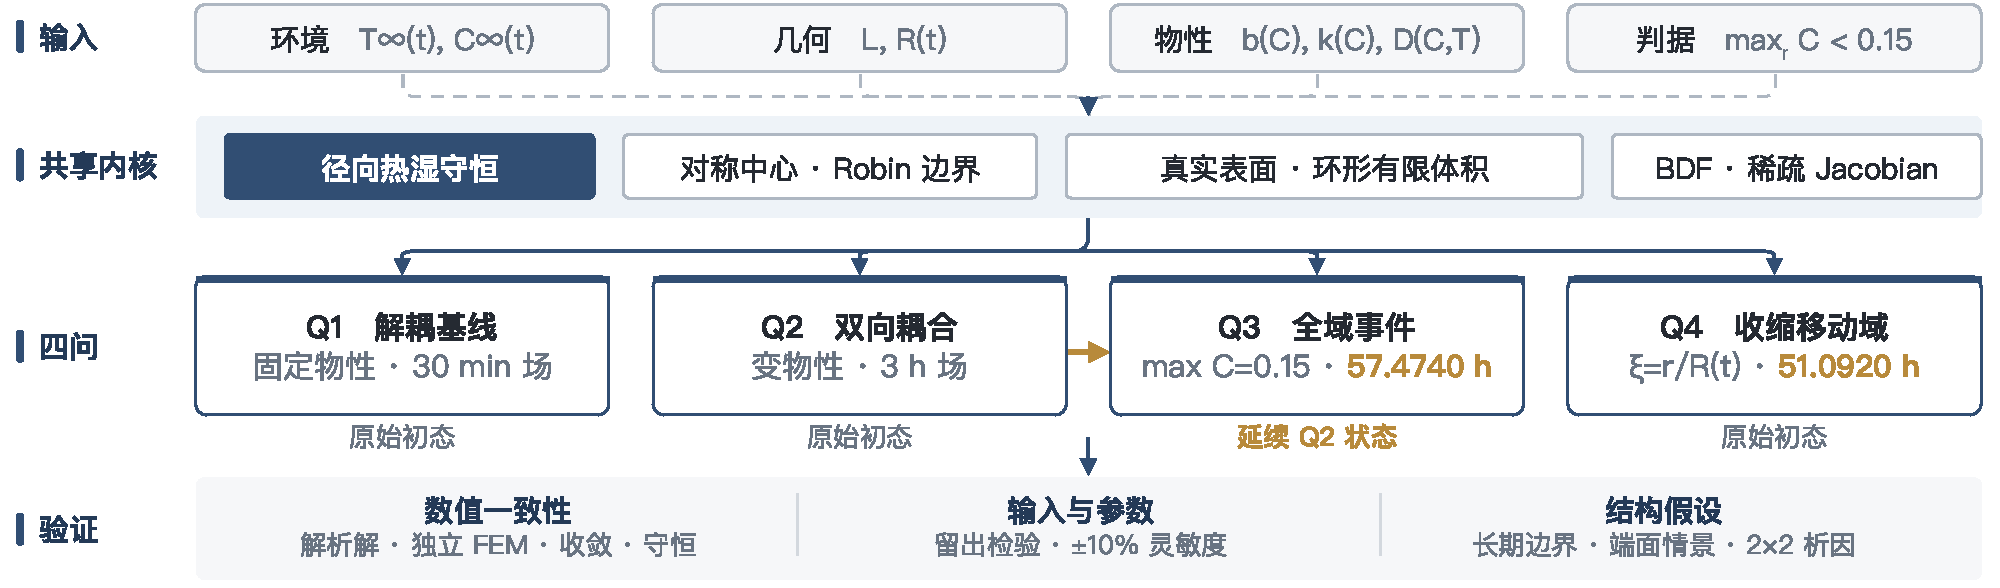
\includegraphics[width=\textwidth]{figures/fig00a_research_roadmap.pdf}
  \caption{四问统一建模与验证框架}
  \label{fig:research-roadmap}
\end{figure}
